\subsection{Hypotheses}
\begin{enumerate}
\item \textbf{Hypothesis 1.} Comparisons of pre and post experiment questionnaires will demonstrate a significant difference in trust scores for overall trust as aggregate measures as well as emotional and analytical trust aggregate measures individually.
1.1 compare pre-post for aggregate trust to show significant difference
1.2 compare pre-post for analytical trust to show a significant difference.
1.3 compare pre-post for emotional trust to show a significant difference.
Make a plot with 3 subplots in this order: overall, analytical, emotional.
\item \textbf{Hypothesis 2.} Comparing the type of trust, WEIRD participants will demonstrate a significant decrease in both analytical and emotional trust in both conditions, with a significant difference between the two types of trust (i.e., emotional and analytical trust will both decrease and differ from each other in magnitude).
2.1 pre-post will be significant in overall trust when looking at just WEIRD participants.
2.2 pre-post will be significant in analytical trust when looking at just WEIRD participants.
2.3 pre-post will be significant in emotional trust when looking at just WEIRD participants.
2.4 compare analytical and emotional standardized change to show a significant difference as predicted by the hypothesis.
Make a plot with 4 subplots in this order: overall, analytical, emotional, emotional-vs-analytical difference.
\item \textbf{Hypothesis 3.} Comparing the type of trust, non-WEIRD participants will demonstrate a significant decrease in analytical and emotional trust in both conditions, with no significant difference between the magnitude of the two types of trust (i.e., emotional and analytical trust will both decrease with no significant difference between each other).
3.1 pre-post will be significant in overall trust when looking at just NORMAL participants.
3.2 pre-post will be significant in analytical trust when looking at just NORMAL participants.
3.3 pre-post will be significant in emotional trust when looking at just NORMAL participants.
3.4 compare analytical and emotional standardized change to show that there is no significant difference as predicted by the hypothesis.
Make a plot with 4 subplots in this order: overall, analytical, emotional, emotional-vs-analytical difference.
\item \textbf{Hypothesis 4.} Group and condition will show distinct effects across trust dimensions and these effects should be visualized in a three-panel grouped-bar figure.
4.1 analytical trust change by Group x Condition with paired pre-post significance markers within each cell.
4.2 emotional trust change by Group x Condition with paired pre-post significance markers within each cell.
4.3 analytical-vs-emotional change difference by Group x Condition with within-condition WEIRD vs NORMAL significance markers.
Recreate the three-panel Group x Condition design and color scheme (Interactive blue, Static/Text orange) with non-overlapping significance annotations.
\end{enumerate}

\section{Results}
\subsection{Hypotheses And Statistical Results}

\subsubsection{Hypothesis 1}
\paragraph{Hypothesis Description.}
Hypothesis 1 predicts a significant pre-post change in reported trust when trust is measured as overall trust and when trust is separated into analytical and emotional components.

\paragraph{Statistical Summary.}
\begin{itemize}
\item 1.1 Overall Trust: $n=504$, $M_{pre}=4.728$, $SD_{pre}=12.319$, $M_{post}=1.062$, $SD_{post}=9.561$, $t(503)=10.395$, $p < .001$, $W=27993.500$, $p_{W} < .001$, $d=-0.463$, $\Delta=-3.667$, sub-hypothesis supported.
\item 1.2 Analytical Trust: $n=504$, $M_{pre}=1.990$, $SD_{pre}=9.439$, $M_{post}=0.661$, $SD_{post}=9.238$, $t(503)=4.854$, $p < .001$, $W=35605.500$, $p_{W} < .001$, $d=-0.216$, $\Delta=-1.329$, sub-hypothesis supported.
\item 1.3 Emotional Trust: $n=504$, $M_{pre}=2.738$, $SD_{pre}=4.309$, $M_{post}=0.401$, $SD_{post}=0.917$, $t(503)=12.796$, $p < .001$, $W=15999.000$, $p_{W} < .001$, $d=-0.570$, $\Delta=-2.337$, sub-hypothesis supported.
\end{itemize}

\paragraph{Tests Used.}
Each pre-post comparison was evaluated with a paired-samples t-test and a Wilcoxon signed-rank test. We also report effect size (Cohen's $d$) and average change ($\Delta$).

\paragraph{Meaning of Results.}
All three trust definitions show significant decreases from pre to post, indicating a robust overall shift in trust and strong support for Hypothesis 1.

\begin{figure}[h]
\centering
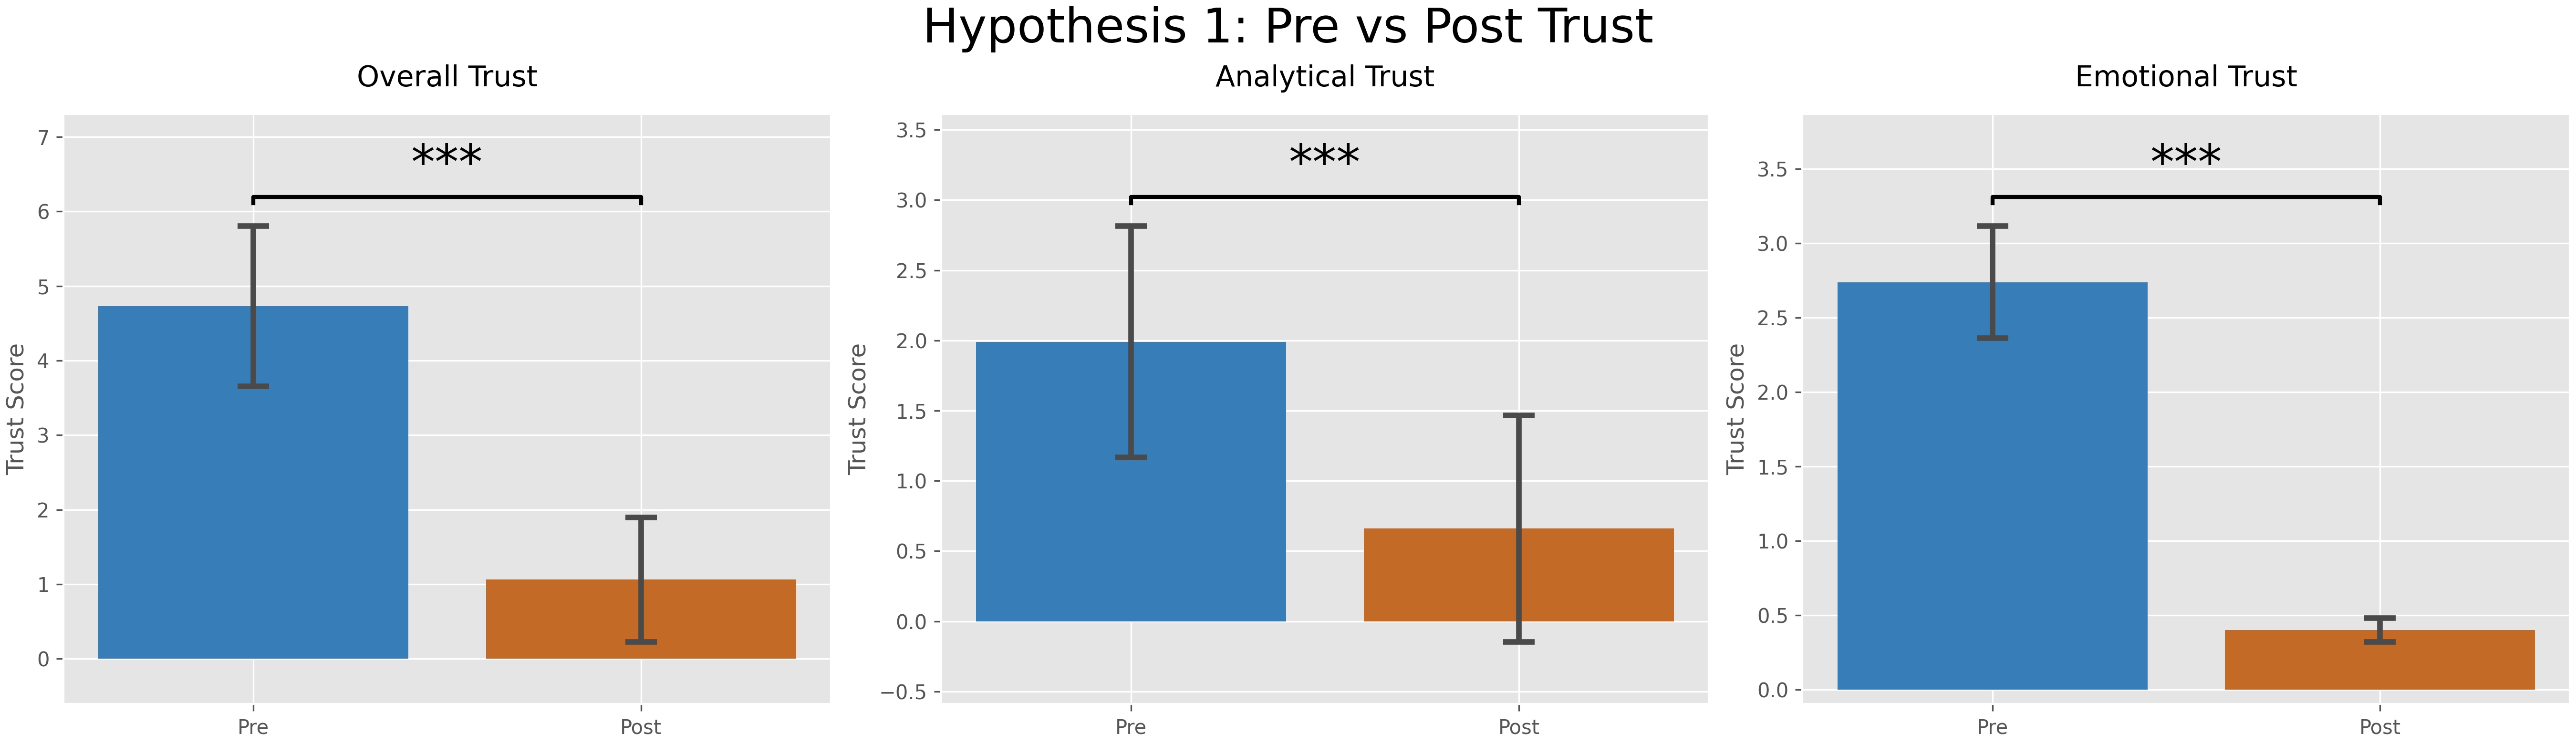
\includegraphics[width=0.85\linewidth]{hypotheses/hypothesis1/hypothesis1.png}
\caption{Visualization for Hypothesis 1.}
\label{fig:hypothesis1}
\end{figure}

\subsubsection{Hypothesis 2}
\paragraph{Hypothesis Description.}
Hypothesis 2 predicts that WEIRD participants will show significant pre-post decreases in overall, analytical, and emotional trust, and that emotional versus analytical standardized change will differ in magnitude.

\paragraph{Statistical Summary.}
\begin{itemize}
\item 2.1 WEIRD Overall pre-post: $n=120$, $M_{pre}=1.217$, $M_{post}=-1.133$, $t(119)=3.440$, $p < .001$, $W=1848.000$, $p_{W} < .001$, $d=-0.314$, $\Delta=-2.350$.
\item 2.2 WEIRD Analytical pre-post: $n=120$, $M_{pre}=-0.167$, $M_{post}=-1.683$, $t(119)=3.014$, $p = .003$, $W=1624.500$, $p_{W} = .003$, $d=-0.275$, $\Delta=-1.517$.
\item 2.3 WEIRD Emotional pre-post: $n=120$, $M_{pre}=1.383$, $M_{post}=0.550$, $t(119)=2.058$, $p = .042$, $W=1936.000$, $p_{W} = .041$, $d=-0.188$, $\Delta=-0.833$.
\item 2.4 WEIRD emotional-vs-analytical standardized change: $n=120$, $M_{em,z}=0.367$, $M_{an,z}=-0.030$, $t(119)=3.301$, $p = .001$, $W=2436.000$, $p_{W} = .002$, $d=0.301$, $\Delta_{z}=0.398$.
\end{itemize}

\paragraph{Tests Used.}
Sub-hypotheses 2.1-2.3 use paired-samples t-tests and Wilcoxon signed-rank tests on pre-post scores. Sub-hypothesis 2.4 uses paired comparison of standardized emotional and analytical change values with both parametric and non-parametric tests.

\paragraph{Meaning of Results.}
The WEIRD subgroup shows significant decreases in all three trust aggregates and a significant difference between emotional and analytical standardized change, supporting Hypothesis 2.

\begin{figure}[h]
\centering
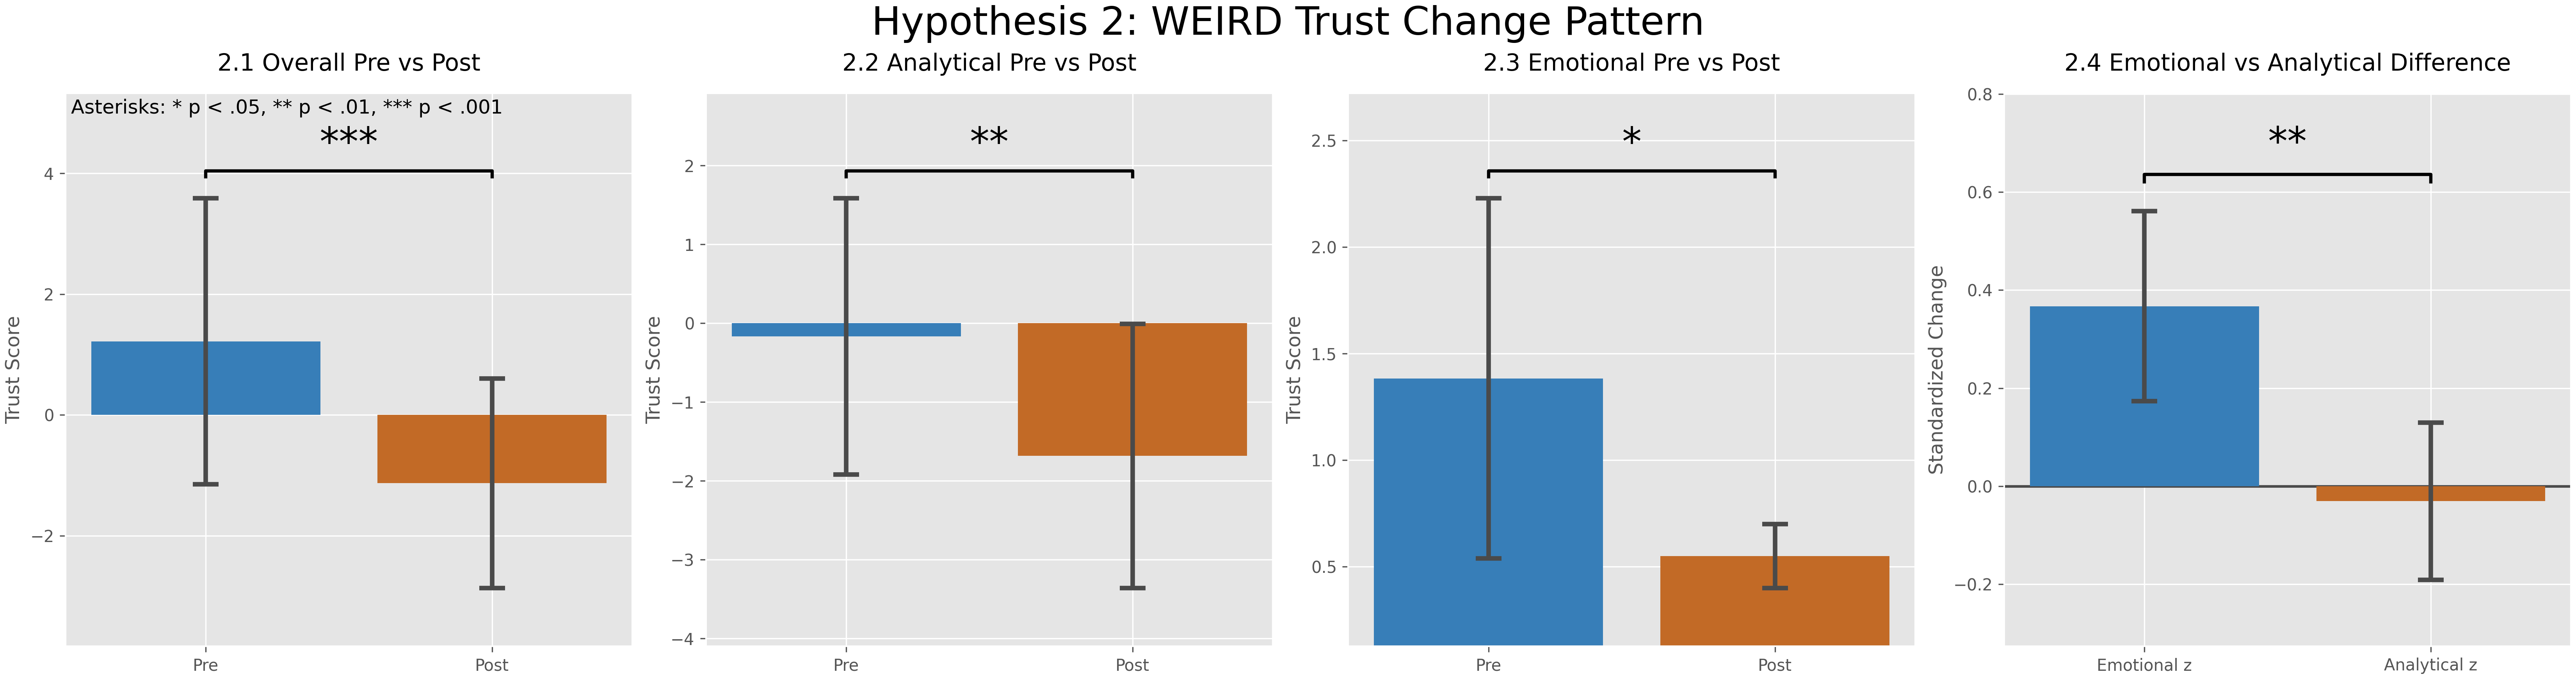
\includegraphics[width=0.85\linewidth]{hypotheses/hypothesis2/hypothesis2.png}
\caption{Visualization for Hypothesis 2.}
\label{fig:hypothesis2}
\end{figure}

\subsubsection{Hypothesis 3}
\paragraph{Hypothesis Description.}
Hypothesis 3 predicts that NORMAL/non-WEIRD participants will show significant pre-post decreases in trust measures, but no meaningful difference in magnitude between emotional and analytical standardized change.

\paragraph{Statistical Summary.}
\begin{itemize}
\item 3.1 NORMAL Overall pre-post: $n=384$, $M_{pre}=5.826$, $M_{post}=1.747$, $t(383)=9.970$, $p < .001$, $W=15536.500$, $p_{W} < .001$, $d=-0.509$, $\Delta=-4.078$.
\item 3.2 NORMAL Analytical pre-post: $n=384$, $M_{pre}=2.664$, $M_{post}=1.393$, $t(383)=3.928$, $p < .001$, $W=21912.000$, $p_{W} = .002$, $d=-0.200$, $\Delta=-1.271$.
\item 3.3 NORMAL Emotional pre-post: $n=384$, $M_{pre}=3.161$, $M_{post}=0.354$, $t(383)=14.183$, $p < .001$, $W=6354.500$, $p_{W} < .001$, $d=-0.724$, $\Delta=-2.807$.
\item 3.4 NORMAL emotional-vs-analytical standardized change: $n=384$, $M_{em,z}=-0.115$, $M_{an,z}=0.010$, $t(383)=-1.923$, $p = .055$, $W=32037.000$, $p_{W} = .024$, $d=-0.098$, $\Delta_{z}=-0.124$.
\end{itemize}

\paragraph{Tests Used.}
Sub-hypotheses 3.1-3.3 use paired-samples t-tests and Wilcoxon signed-rank tests for pre-post comparisons. Sub-hypothesis 3.4 compares standardized emotional and analytical change with both a paired t-test and Wilcoxon signed-rank test.

\paragraph{Meaning of Results.}
NORMAL/non-WEIRD participants show clear pre-post decreases in overall, analytical, and emotional trust. For emotional-versus-analytical standardized change, the t-test is non-significant while the Wilcoxon test is significant, indicating mixed but small-magnitude evidence for this contrast.

\begin{figure}[h]
\centering
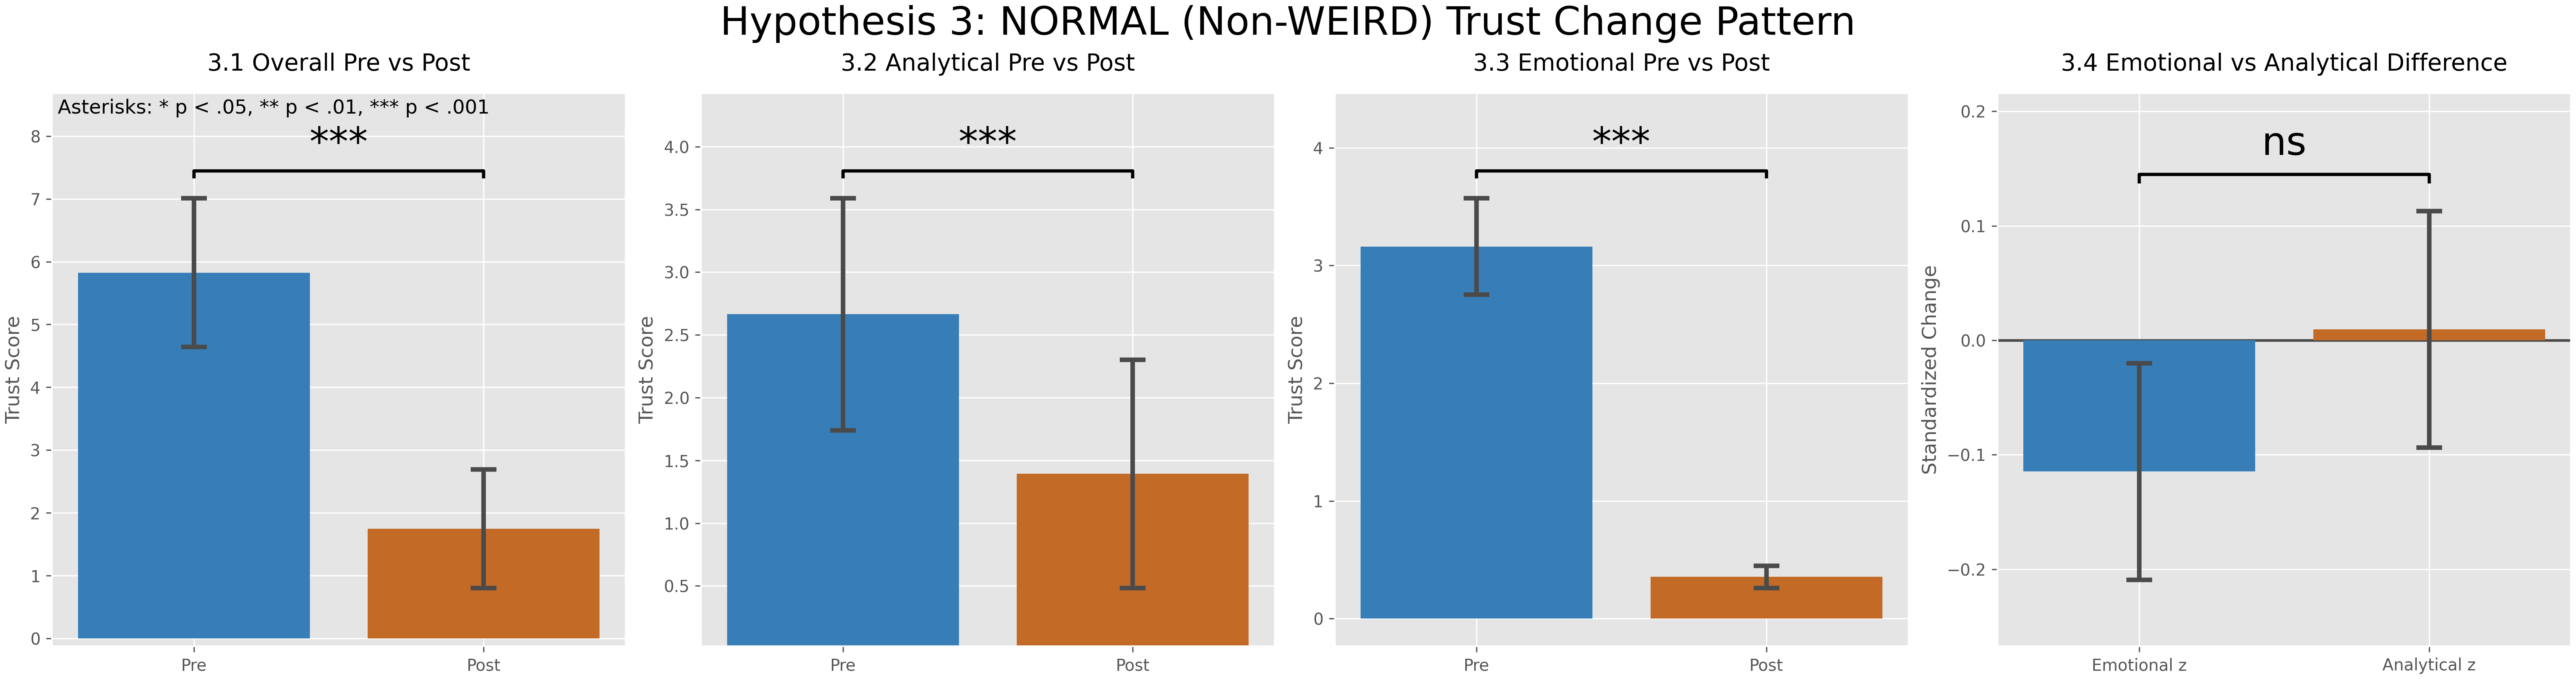
\includegraphics[width=0.85\linewidth]{hypotheses/hypothesis3/hypothesis3.png}
\caption{Visualization for Hypothesis 3.}
\label{fig:hypothesis3}
\end{figure}

\subsubsection{Hypothesis 4}
\paragraph{Hypothesis Description.}
Hypothesis 4 evaluates whether group (WEIRD vs NORMAL) and condition (Interactive vs Static/Text) produce distinct effects across three trust-change dimensions in a three-panel Group $\times$ Condition design. All trust-change outcomes are computed as per-item average change (Post - Pre).

\paragraph{Statistical Summary.}
\begin{itemize}
\item 4.1 Analytical trust change by Group $\times$ Condition (left panel): paired pre-post tests were WEIRD / Interactive: $t(59)=2.17$, $p = .034$, $\Delta M=-0.180$; WEIRD / Static (Text): $t(59)=2.14$, $p = .037$, $\Delta M=-0.123$; NORMAL / Interactive: $t(191)=2.81$, $p = .006$, $\Delta M=-0.130$; NORMAL / Static (Text): $t(191)=2.74$, $p = .007$, $\Delta M=-0.124$. Omnibus four-cell ANOVA: $F=0.14$, $p = .938$. Interaction estimate: $b=-0.050$, $t(500)=-0.39$, $p = .696$.
\item 4.2 Emotional trust change by Group $\times$ Condition (middle panel): paired pre-post tests were WEIRD / Interactive: $t(59)=1.71$, $p = .092$, $\Delta M=-0.104$; WEIRD / Static (Text): $t(59)=1.22$, $p = .229$, $\Delta M=-0.081$; NORMAL / Interactive: $t(191)=9.48$, $p < .001$, $\Delta M=-0.297$; NORMAL / Static (Text): $t(191)=10.57$, $p < .001$, $\Delta M=-0.326$. Omnibus four-cell ANOVA: $F=7.49$, $p < .001$. Interaction estimate: $b=-0.051$, $t(500)=-0.55$, $p = .585$.
\item 4.3 Analytical-vs-emotional change difference by Group $\times$ Condition (right panel): Welch tests by condition were Interactive: $t=-2.28$, $p = .025$, $M_{WEIRD}=-0.076$, $M_{NORMAL}=0.167$; Static (Text): $t=-2.46$, $p = .015$, $M_{WEIRD}=-0.042$, $M_{NORMAL}=0.202$. Omnibus four-cell ANOVA: $F=3.82$, $p = .010$. Interaction estimate: $b=0.001$, $t(500)=0.01$, $p = .996$.
\end{itemize}

\paragraph{Tests Used.}
This hypothesis combines multiple tests: paired pre-post tests within each Group $\times$ Condition cell, Welch independent-samples tests for between-group contrasts within condition (Panel 4.3), omnibus four-cell ANOVAs, and regression-based interaction estimates.

\paragraph{Meaning of Results.}
The pattern suggests robust trust-change effects within several cells and clear between-group differences in the analytical-vs-emotional difference metric, but no reliable Group $\times$ Condition interaction in the regression interaction terms. This indicates stronger main-pattern differences than condition-specific moderation.

Asterisk key: * $p < .05$, ** $p < .01$, *** $p < .001$.

\begin{figure}[h]
\centering
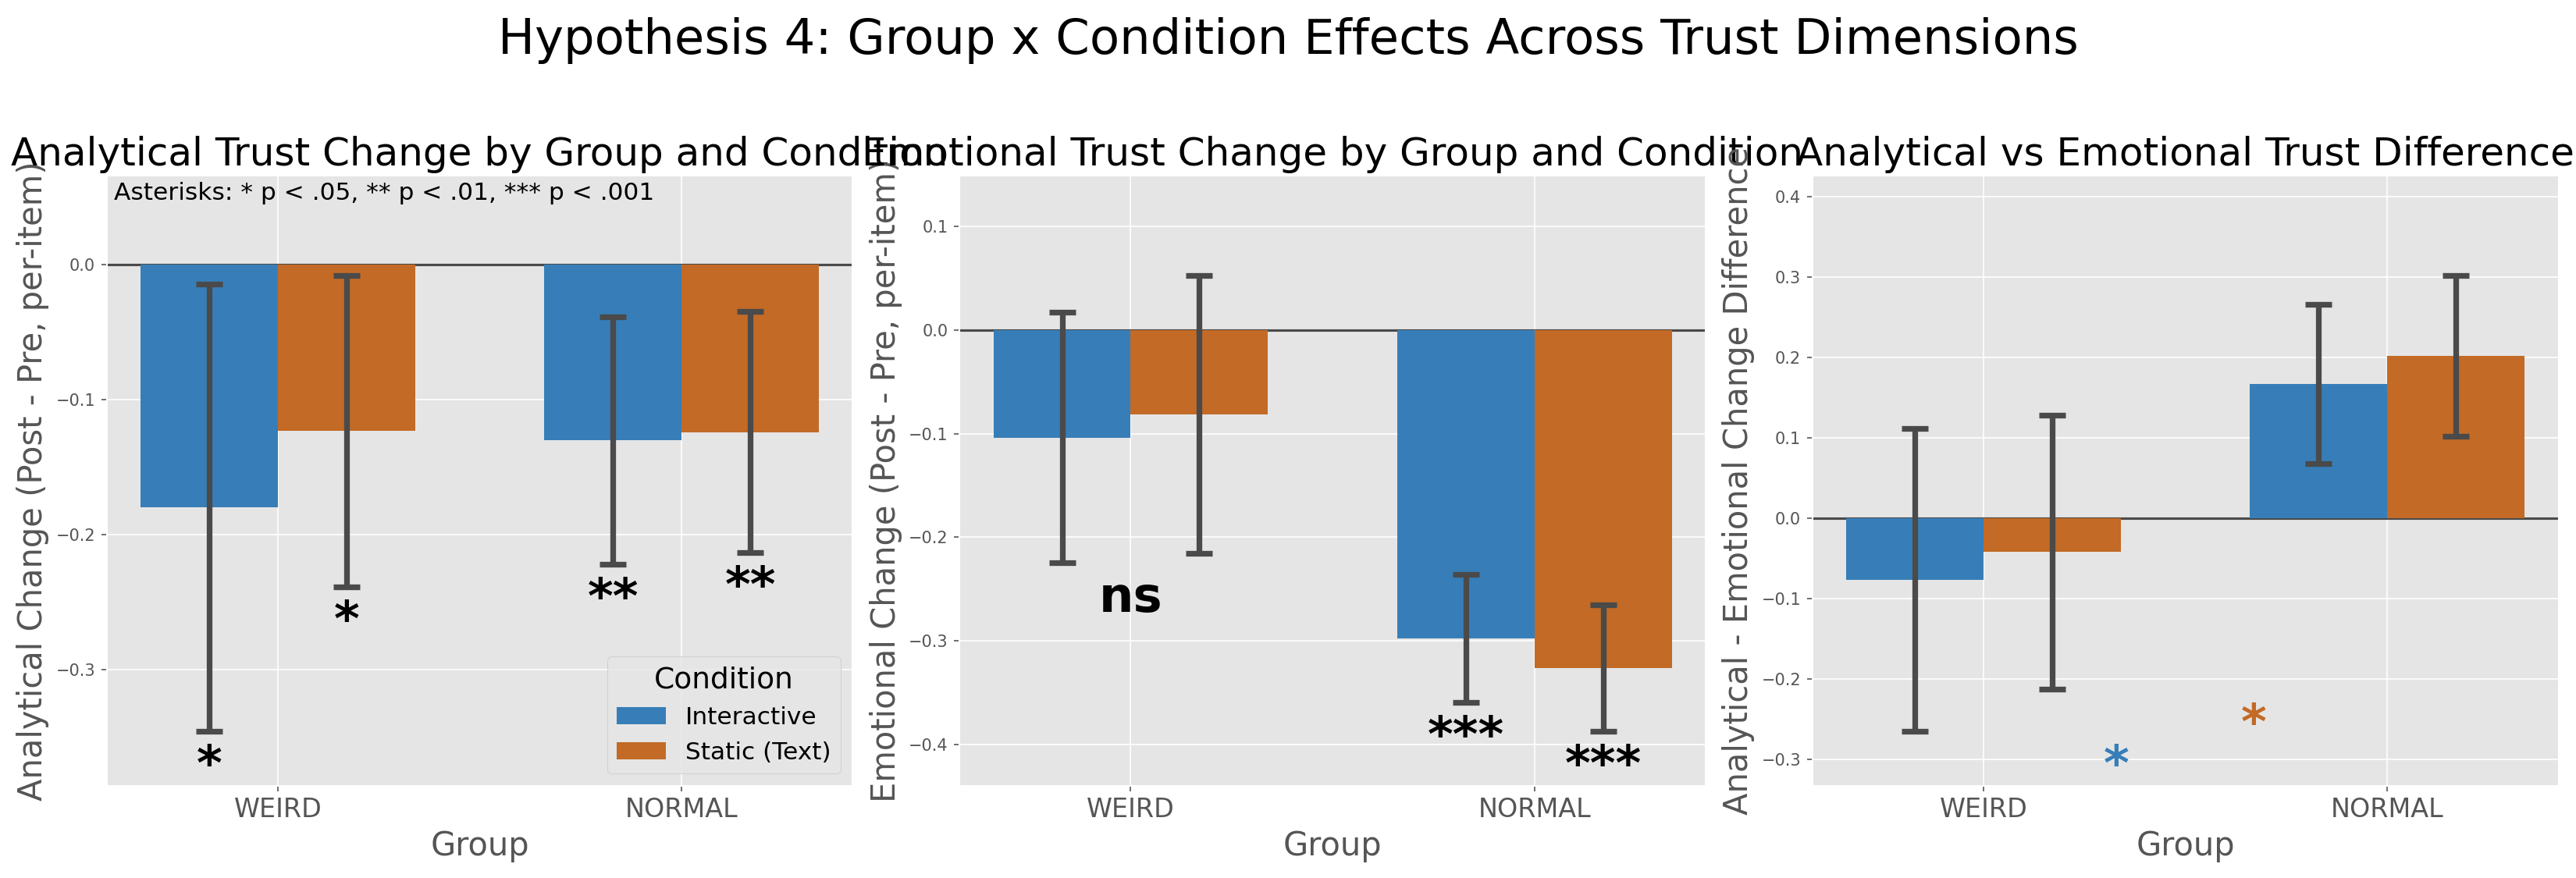
\includegraphics[width=0.85\linewidth]{hypotheses/hypothesis4/hypothesis4.png}
\caption{Visualization for Hypothesis 4.}
\label{fig:hypothesis4}
\end{figure}

